\chapter{Physics: Phase transitions}

In \chref{ch:statphys} we saw that in a statistical mechanical system,
observables of interest can be derived from the free energy or grand potential,
i.e. from $\log\mathcal{Z}$. During this discussion there was more or less an
assumption that $\log\mathcal{Z}$ was mathematically well behaved, or at least
I never brought it up. In general $\log\mathcal{Z}$ may not be smooth
everywhere. A point in the space of control parameters where $\log\mathcal{Z}$
is not well behaved is a {\it critical point}\index{critical point}. Depending
on the system under study, this may even be extended to a {\it critical line} or
{\it critical surface}; generically we refer to these as {\it phase
boundaries}\index{phase boundary}. These shapes separate the space of control parameters
into different regions where $\log\mathcal{Z}$ is analytic. Each of these
regions corresponds to a {\it phase}\index{phase} or {\it state}\index{state} of
the system. Physically, the system exhibits qualitative differences between
different phases. When the system crosses this critical boundary and moves from
one phase to another, it is said to undergo a {\it phase transition}\index{phase
transition}.
Much of our current understanding of phase transitions was developed by studying
liquid-gas systems and ferromagnets. 

Critical temperatures in fluids were discovered by T. 
Andrews\footnote{He seems to be the one who coined the
term ``critical point".}~\cite{andrews_bakerian_1869}.
J. D. van der Waals\footnote{Apparently, van der Waals grew up working
class, which at that time in Amsterdam precluded him from attending
university. As a result, he started off as a school teacher and did not
obtain his PhD until he was in his late 30s. His PhD thesis seems to be
the work that won him the 1910 Nobel prize.}
was, to my knowledge, the first to attempt to
model the existence of criticality~\cite{van_der_waals_over_1873}.
Beginning with such work, analyses of critical singularities 
focused largely on static properties, such as equilibrium
expectation values. However it is also the case that dynamical properties,
such as transport coefficients and responses to time-dependent perturbations,
which cannot be derived from the equilibrium distribution, also contain
critical behavior. In this context one can distinguish between
\index{critical phenomena}
{\it static critical phenomena} and {\it dynamic critical phenomena}.

These research notes were made from the perspective of a researcher working
in lattice field theory, and one advantage of the lattice, which will be
discussed later in \chref{ch:preliminaries}, is that it allows one
to make direct analogies with statistical mechanical systems, and in
particular, to utilize powerful techniques like renormalization group (RG)
analysis. On the lattice, one is dealing with the equilibrium distribution,
and hence we will restrict our attention to only static critical 
phenomena\footnote{If you want to learn about dynamic critical phenomena, a very
friendly introduction can be found in Ref.~\cite{halperin_theory_2019}.
A landmark paper introduces the classification system for dynamical
critical phenomena is Ref.~\cite{hohenberg_theory_1977}.}.

This chapter will generally try to follow 
lectures by F. Karsch, as well as the book by Binney et
al.~\cite{binney_theory_1992}. 

\section{Types of transitions}

\begin{figure}
\centering
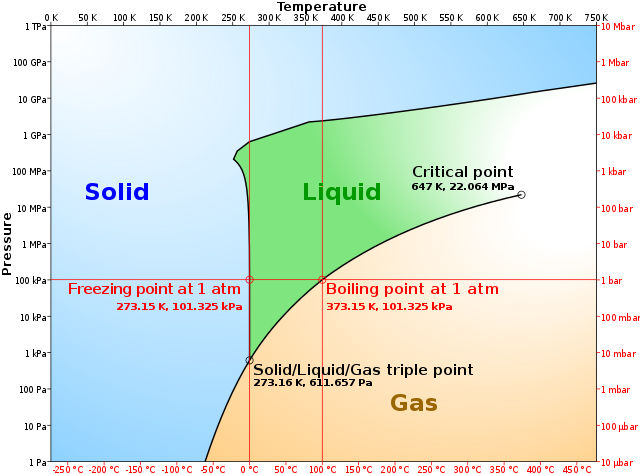
\includegraphics[width=\linewidth]{figs/simplified_water.png}
\caption{Simplified phase diagram for water indicating its solid, liquid, and
gas phases. Phase boundaries are indicated by the black lines. It is difficult
to see on the scale of this plot, but the solid-liquid boundary near 1 atm has a
slight lean to the left, which is an uncommon feature for most substances having
a solid-liquid transition. Beyond the
critical point, liquid and gas phases cannot be distinguished. 
Image taken from Wikipedia \cite{Wiki_water}.}
\label{fig:phase_water}
\end{figure}

The definition of phase transition given in the introduction is mathematically
unambiguous, but it may not help give much physics intuition. To this end, it is
useful to think about some archetypical substances that exhibit many of the
properties common to systems undergoing phase transitions.

In \figref{fig:phase_water} we see a simplified {\it phase diagram}\index{phase
diagram} for water. A phase diagram shows the various phases where
the free energy is analytic, separated by phase boundaries as discussed before.
Phase transitions can be classified according to how the free energy and its
derivatives behave when crossing a phase boundary. In the case of water, these
are {\it first-order}\footnote{This naming scheme dates back to Paul Ehrenfest's
classification of phase transitions. Under his scheme, a transition is said to
be of order $n$ if the $n\nth$ derivative of the free energy is discontinuous
across the phase boundary.} phase transitions\index{phase transition!first-order}.
In general when changing a control parameter, one has to dump energy into the
system; for instance increasing temperature generically requires the addition of
heat. When the system hits a first-order phase boundary, energy dumped into the
system will, for a brief period, not change the control parameter, and instead
is needed to change the phase of the substance. In the case of water, when
hitting for instance the solid-liquid first-order line, additional heat is used
to break the bonds between molecules, changing the substance from a solid into a
liquid. The energy required to do this is the {\it latent heat}\index{latent
heat}. The existence of a latent heat defines first-order phase transitions.

Along phase boundaries, different phases may coexist. For instance along the
solid-liquid phase boundary one will in general find a mixture of solids and
liquid, which is sometimes called a {\it slurry}\index{slurry}. We also use
the common verbiage when crossing the boundaries: the substance {\it
melts}\index{melt} when going from solid to liquid, {\it
evaporates}\index{evaporate} when going
from liquid to gas, and {\it sublimates}\index{sublimate} when going from solid
to gas. Salient in \figref{fig:phase_water} is also a critical point, beyond
which liquid and gas cannot be distinguished. One sometimes refers to this
region as a {\it supercritical fluid}\index{supercritical fluid}. A path from
liquid to gas region going around the critical point, not crossing any phase
boundary, allows for a analytic change from liquid to gas. Such a change of
phase is referred to as a {\it crossover}\index{crossover}. Since this change is
completely analytic, we will distinguish crossovers from phase transitions in
these notes. 

\begin{figure}
\centering
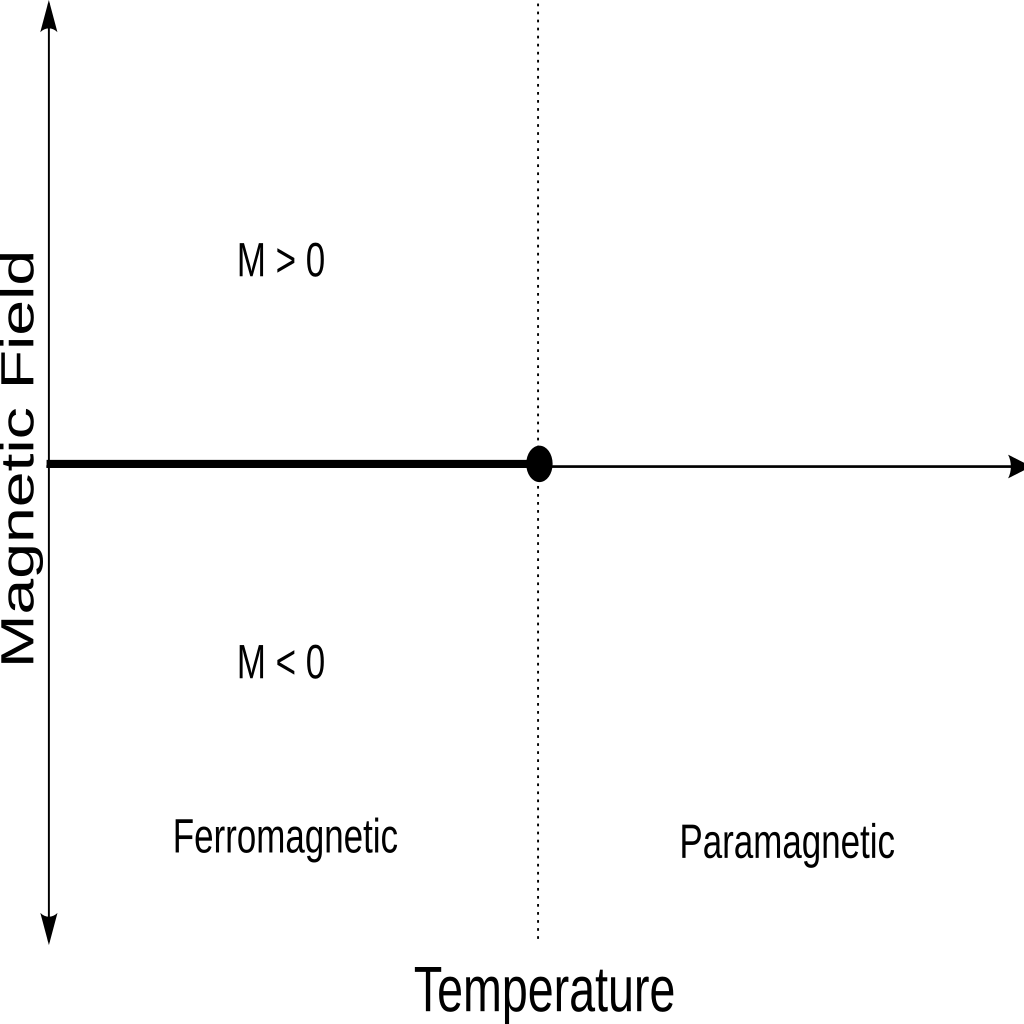
\includegraphics[width=\linewidth]{figs/ising_phase_diagram.png}
\caption{Phase diagram for the 2-$d$ Ising model. The solid black
circle indicates the critical temperature; the solid line connected to it is a
first-order line. Magnetization is indicated by $M$.
Image taken from Ref.~\cite{ising_picture}.}
\label{fig:phase_ising}
\end{figure}

Water gives the quintessential example of a first-order phase transition. Now we
will consider {\it second-order} or {\it continuous} phase
transitions\index{phase transition!second-order}\index{phase
transition!continuous}. The Ising model of a ferromagnet in two or more
dimensions is the quintessential example for second-order transitions.
The 2-$d$ {\it Ising model}\index{Ising model} 
imagines a magnet as being comprised of interacting spins
with nearest-neighbor interactions. Its Hamiltonian is
\begin{equation}
H=-J\sum_{\ev{i j}} \sigma_i \sigma_j-h \sum_j
\sigma_j,
\end{equation}
where the brackets indicate a sum over nearest-neighbors,
$\sigma_i\in\{+1,-1\}$ indicates the value of spin $i$, $h$ gives the
coupling of the spins to an external magnetic field, and $J$ gives the
nearest-neighbor interaction strength.

The Ising model phase diagram in two dimensions is given 
in \figref{fig:phase_ising}.
At fixed temperature, when varying the external magnetic field, one can
discontinuously flip the magnetization $M$. Moving from left to right in $T$
at $h=0$, this first-order line terminates in a second-order critical point. When
approaching the critical point by varying the temperature, one can
show\footnote{This was first done by Onsager~\cite{onsager_crystal_1944}. A
nice, closed-form solution like this is not available for three dimensions or
more. Critical exponents are typically extracted from Monte Carlo simulations.}
that the magnetization changes as
\begin{equation}\label{eq:exampleCP}
  M\sim|T-T_c|^\beta
\end{equation}
with $\beta=1/8$. This sort of behavior is a hallmark of second-order
transitions. The quantity $\beta$ is an example of a {\it critical
exponent}\index{critical exponent}. 
Many other physical quantities will also exhibit asymptotic behavior when
approaching a second-order point analogous to \equatref{eq:exampleCP}.
These will have their own critical exponents. These
critical exponents can be related to each other, which we discuss
in \secref{sec:scalingHypothesis}.

What is positively remarkable is that completely different
physical systems sometimes have exactly the same critical exponents.
This phenomenon is known as {\it universality}\index{universal}, and when two
systems have the same exponents, they are said to belong to the same {\it
universality class}\index{universality class}. In the context of lattice QCD,
it has for example been demonstrated that the chiral transition for $N_f=2+1$
quark masses in the chiral limit $m_u=m_d\equiv m_l\to0$ belongs to the 3-$d$, 
$\ON(4)$ universality class~\cite{ding_chiral_2019}, 
the same class as a generalized magnet with spins
free to rotate on 4-$d$ hyperspheres.

For the Ising model, at extremely high temperatures, 
the $TS$ term in the free energy dominates over
the internal energy, and the spins of the ferromagnet become, in the absence of
an external magnetic field, randomly aligned\footnote{In the high-temperature
phase, one can point the spins in a particular direction by applying an external
field.}, and hence the net magnetization is zero. If one decreases the
temperature below $T_c$, the internal energy coming from spin alignment becomes
more important, and domains of aligned spins start to emerge. Eventually the
system will settle pointing in one direction. There is nothing special about the
direction the system picks; this is an example of spontaneous symmetry
breaking\index{spontaneous symmetry breaking}, which plays a major role in QFT,
as discussed in \secref{sec:ssb}. 

\section{The Lee-Yang theorem}\label{sec:leeyang}\index{Lee-Yang!Theorem}

One of the lessons of \chref{ch:statphys} is that the partition function of a
system determines all its observables. For example in the grand canonical
formulation, we saw that the grand potential is related to the partition
function by
\begin{equation}\label{eq:grandPotZ}
  \Phi\left(V,T,\vec{\mu}\right)=-T\log\grandZ.
\end{equation}
Remaining observables, such as energy densities, entropy, heat capacity, and so
on, can then in principle be determined by carefully taking partial derivatives
and utilizing relations like the first law of thermodynamics or the Gibbs-Duhem
relation.


\begin{figure} 
\centering
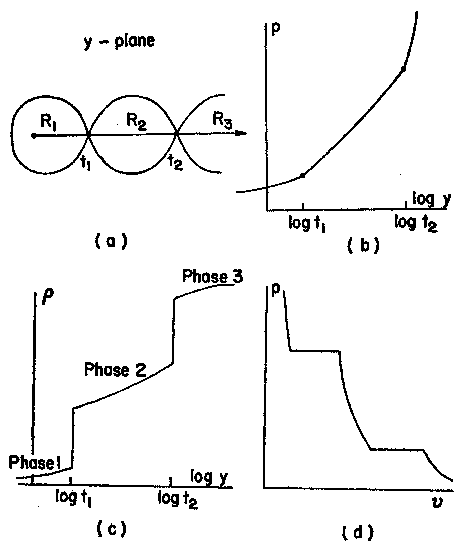
\includegraphics[width=\linewidth]{figs/lee_yang.pdf}
\caption{
Figure from Ref.~\cite{yang_statistical_1952}. In their setup, they consider a
three-phase system. $y$ is the fugacity, so $\log y\sim \mu/T$. The pressure is
$p$; $t_1$ and $t_2$ are zeros of the partition function, and $\rho$ is a
$\mu$-derivative of the pressure.
}
\label{fig:leeYangTheorem}
\end{figure}


The partition function is also useful to find
phase transitions. Perhaps the most important work in this regard is by Lee and
Yang~\cite{yang_statistical_1952}, who demonstrated that, in the 
{\it thermodynamic limit}\index{limit!thermodynamic} limit, i.e.
$V\to\infty$, $\grandZ(h)$, which we write as a function of the magnetization or
symmetry-breaking parameter $h$, will have zeros at phase transitions. According
to \equatref{eq:grandPotZ} then, we correspondingly expect singularities in the
free energy. 
In their original paper, they allow the fugacity, which they denote
as $y$, to be complex, then imagine the situation in the complex plane.
The regions of analyticity for $y$ along with the expected behavior
of the pressure and its $\mu$-derivatives is shown schematically
in \figref{fig:leeYangTheorem}, which is taken from Lee and Yang. 


\begin{figure} 
    \centering
    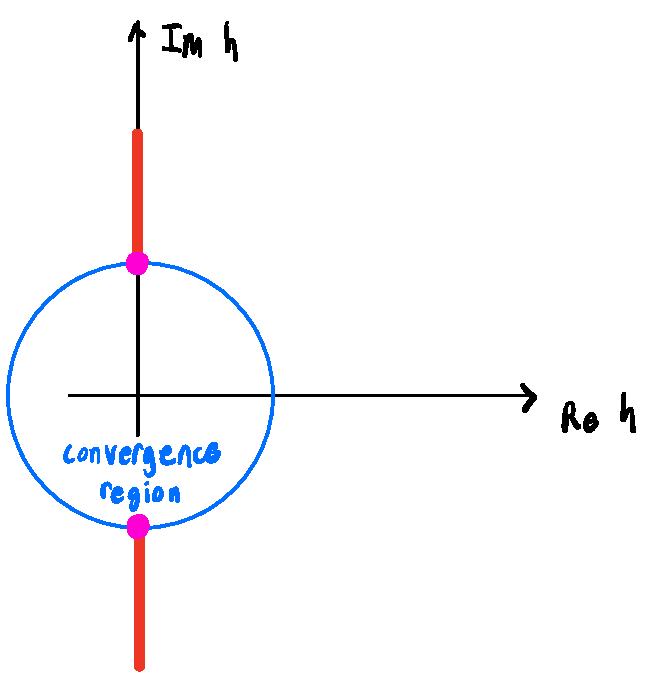
\includegraphics[width=\linewidth]{figs/LYE.pdf}
    \caption{
        Generic singularity structure of the Ising model partition function in the
        complex $h$ plane, for $T<T_c$ in the thermodynamic limit.
    }
    \label{fig:LYE}
\end{figure}


The above logic is what happens exactly at the critical point $T=\Tc$ and $h=0$.
When we are away from the critical point, the situation in the complex plane
changes somewhat. Still in the thermodynamic limit, let us imagine $T<\Tc$ 
and let $h$ be complex. The expectation is that $\log Z(h)$ should
have two branch cuts in the complex-$h$ plane, called 
{\it Lee-Yang edges}\index{Lee-Yang!edge}, that terminate at
branch points called {\it Lee-Yang edge singularities}.
This is shown schematically in \figref{fig:LYE}. The expectation is
that, as $T\to\Tc$, these branch points will approach and eventually
pinch the real axis, where they manifest as a phase transition
in accordance with the Lee-Yang theorem.

As shown in \figref{fig:LYE}, the Lee-Yang edges should limit the convergence
radius of $\log Z$. In principle there are other singularities possible.
The {\it extended analyticity conjecture}\index{extended analyticity conjecture}
posits that the Lee-Yang edges should be the closest singularities
to the origin in the complex $h$-plane~\cite{fonseca_ising_2003}. 


\section{The scaling hypothesis}\label{sec:scalingHypothesis}
All critical exponents\index{critical exponent} can be written as functions 
of the number of dimensions $d$ as well as $\nu$ and $\eta$. Given the reduced 
temperature\index{temperature!reduced}
\begin{equation}
  t\equiv\frac{T-T_c}{T_c}
\end{equation}
and external magnetic field $h$ one gets the 
relationships~\tabref{tab:scaling}.
These are equivalent to the {\it hyperscaling relations}
\index{hyperscaling relation}
\begin{equation}\begin{aligned}
2\beta+\gamma&=2-\alpha,\\
2\beta\delta-\gamma&=2-\alpha,\\
\gamma&=\nu(2-\eta),\\
\nu d&=2-\alpha.
\end{aligned}\end{equation}
These can be derived from the {\it scaling hypothesis}\index{scaling
hypothesis}, which we will now show for a large class of RG transformations.
\begin{table}
\begin{tabularx}{\linewidth}{lCr} \hline\hline
       Exponent & Definition & Value\\[3pt]\hline
$\alpha$ & $C_V\sim|t|^{-\alpha}$  & $2-\nu d$\\[3pt] 
$\beta$ & $m\sim|t|^{\beta}$ & $\frac{1}{2}\nu(d+\eta-2)$\\[3pt]
$\gamma$ & $\chi\sim|t|^{-\gamma}$  & $\nu(2-\eta)$\\[3pt] 
$\delta$ & $m\sim h^{1/\delta}$ &  $\frac{d+2-\eta}{d-2+\eta}$\\[3pt]
$\nu$ & $\xi\sim |t|^{-\nu}$ & \\[3pt]
        \hline\hline
\end{tabularx}
\caption{Relationships among the critical exponents. Table adapted from 
         from Ref.~\cite{binney_theory_1992}. In each case one coupling is
         small while the other is fixed to zero. For $\beta$, $t$ approaches
         zero from below.}
\label{tab:scaling}
\end{table}

Suppose we start with a system of variables $\set{\sigma}$ with Hamiltonian $H$
and $n$ couplings $\vec{k}=(k_1,...,k_n)^t$. After one RG step, we obtain
a new system of spins $\set{\sigma'}$ with $H'$ and $\vec{k}'$. We want
that expectation values remain unchanged after an RG step.
Thinking about block transformations in particular, one can
achieve this by collecting 
all those original configurations $\set{\sigma}$ that lead to the same
renormalized configuration $\set{\sigma'}$\footnote{For example in the 2$d$
Ising model, if one blocks three up-spins and one down spin, there are 
four possible ways to get the same effective spin via majority rule.}, which can be
summarized as
\begin{equation}
  e^{-H'\left(\set{\sigma'},~\vec{k}'\right)}
     =e^{-\beta G(\vec{k})}\sum_{\set{\sigma}~
                        {\rm giving}~\set{\sigma'}}
      e^{-H\left(\set{\sigma},~\vec{k}\right)}.
\end{equation}
Here we have expressed an overall normalization as $e^{-\beta G}$, which will
be convenient later. When we sum over all $\set{\sigma'}$ we then get
\begin{equation}
  Z'(\vec{k}')=e^{-\beta G(\vec{k})} Z(\vec{k}),
\end{equation}
or in terms of free energies,
\begin{equation}
  F'(\vec{k}')=F(\vec{k})-G(\vec{k}).
\end{equation}
Now $F$ is extensive, so we can write
\begin{equation}
  F(\vec{k})=Nf(\vec{k})
\end{equation}
where $N$ is the number of spins on the original lattice and $f$ is intensive.
Similarly one can write
\begin{equation}
  F'(\vec{k}')=\frac{N}{b^d}f(\vec{k}')~~~~\text{and}~~~~G(\vec{k})=Ng(\vec{k}),
\end{equation}
where $b$ is the {\it scale factor}\index{scale factor}, which represents the
factor by which the lattice spacing changes. That $F$ and $F'$ are proportional
to the same intensive function with different couplings follows from the fact
that the effective Hamiltonian $H'$ has the same functional form as $H$.
Hence
\begin{equation}\label{eq:widom1}
f(\vec{k}')=b^d\left(f(\vec{k})-g(\vec{k})\right).
\end{equation}


Next, let's think about how to relate the couplings $\vec{k}'$ and $\vec{k}$
near the fixed point $\vec{k}_0$. 
We can Taylor expand the renormalization action $\vec{R}$ in the vicinity of $\vec{k}_0$ to find
\begin{equation}
  \vec{k}_0+\delta\vec{k}'=\vec{R}\left(\vec{k}_0+\delta\vec{k}\right)
                          \approx\vec{R}(\vec{k}_0)
                           +\frac{\partial R_i(\vec{k})}{\partial k_j}
                              \Big|_{\vec{k}=\vec{k}_0}\delta\vec{k}.
\end{equation}
The first-order term defines a matrix $M$.
Since the effect of the renormalization action
$\vec{R}$ on the fixed point is $\vec{R}(\vec{k}_0)=\vec{k}_0$, we can write
\begin{equation}
  \delta\vec{k}'=M\delta\vec{k}.
\end{equation}
Now let's switch to a basis in which $M$ is diagonal. In this basis, our
original system contains new couplings $\vec{x}$, and hence the renormalized
couplings $\vec{x}'$ are given according to the eigenvalues of $M$ as
\begin{equation}
  x_i'=\lambda_i x_i~~~~\text{no summation}.
\end{equation}
Hence we can recast \equatref{eq:widom1} as
\begin{equation}
f(\lambda_1x_1,\lambda_2x_2,...)=b^d\left(f(x_1,x_2,...)-g(x_1,x_2,...)\right).
\end{equation}


Now $f$ and $g$ are some kinds of functions of $\vec{x}$. Generally speaking
there will be some part that is expressible as a Taylor series in the $\vec{x}$;
this is called the {\it regular} part.\index{regular} There must also be some
part not expressible as a Taylor series in order that we can obtain the power
law behavior one finds in the vicinity of a phase transition; this is
called the {\it singular} part.\index{singular} In order to proceed we make
the following assumption: The singular part is completely contained in
$f$. This is not true of all RG transformations, but it is true
of many; for example it can be shown that this assumption holds for any
RG transformation whose renormalized block variables depend linearly
on the original ones. Under this assumption we can write
\begin{equation}
  \fsing(\lambda_1x_1,\lambda_2x_2,...)=b^d\fsing(x_1,x_2,...).
\end{equation}


Finally we specialize to our couplings $t$ and $h$. Sufficiently close to the
critical point, these can be identified with two of these eigendirections, say
$x_1=t$ and $x_2=h$. Furthermore the action of the RG transform will not abruptly
change the direction of the flow; this is equivalent to $\lambda_t>0$ and
$\lambda_h>0$. Since these eigenvalues are positive and $b$ is positive we
can introduce $\lambda_i=b^{\,y_i}$. Hence,
\begin{equation}
  \fsing(b^{\,y_t}t,b^{\,y_h}h,...)=b^d\fsing(t,h,...).
\end{equation}
Since the system is supposed to be scale-invariant, you are free to choose $b$
as you like; e.g. you are free to set the length scale of your blocking
procedure in your RG step. Hence we can choose
\begin{equation}
  b=|t|^{-1/y_t}~~~~\text{or}~~~~b=h^{-1/y_t}.
\end{equation} 
If we restrict our attention to the critical surface $x_i=$ for all $i\geq2$
we obtain finally the scaling hypothesis:\index{scaling hypothesis!Widom}
\begin{theorem}{Widom scaling hypothesis}{}
  \begin{equation*}\begin{aligned}
    \fsing(t,h)&=|t|^{d/y_t}\fsing\left(\pm1,|t|^{-y_h/y_t}h\right)\\
    \fsing(t,h)&=h^{d/y_h}\fsing\left(h^{-y_t/y_h},1\right)
  \end{aligned}\end{equation*}
\end{theorem}

One can see from the scaling hypothesis that the order parameter, its
susceptibility, and $C_V$ will scale according to critical exponents
near the critical point. We choose one or the other of the above forms
strategically depending on the observable we're looking at:
\begin{equation}\begin{aligned}
  C_V&=\partial_T^2 F
     \sim\partial_t^2 |t|^{d/y_t}\fsing\left(\pm1,|t|^{-y_h/y_t}h\right)
     \sim|t|^{d/y_t-2}
     \equiv|t|^{-\alpha}\\
  m\big|_{h=0}&=\partial_h F\big|_{h=0}
     \sim\partial_h |t|^{d/y_t}\fsing\left(\pm1,|t|^{-y_h/y_t}h\right)\big|_{h=0}
     \sim|t|^{d/y_t-y_h/y_t}
     \equiv|t|^{\beta}\\
  \chi\big|_{h=0}&=\partial^2_h F\big|_{h=0}
     \sim\partial^2_h |t|^{d/y_t}\fsing\left(\pm1,|t|^{-y_h/y_t}h\right)\big|_{h=0}
     \sim|t|^{d/y_t-2y_h/y_t}
     \equiv|t|^{-\gamma}\\
  m\big|_{t=0}&=\partial_h F\big|_{t=0}
     \sim h^{d/y_h}\fsing\left(h^{-y_t/y_h},1\right)\big|_{t=0}
     \sim h^{d/y_h-y_t/y_h}
     \equiv h^{1/\delta}.
\end{aligned}\end{equation}
One can eliminate the unknown variables $y_h$, $y_t$, and $d$ to obtain
the first two hyperscaling relations.

\subsection{Finite size scaling}\index{finite size scaling}

In \secref{sec:leeyang} we saw that phase transitions happen in the $V\to0$
limit. However when looking at real-word, condensed-matter systems, we deal
exclusively with finite volumes. Similarly all lattice calculations are on
configurations stored in computer memory, and are hence themselves finite as
well. On the other hand, we would like our understanding of statistical physics
to say something about the real, finite-volume world, and conversely, we would
like to learn about phase transitions of large systems from finite-volume
lattice calculations. How do we reconcile these seemingly conflicting goals?
This is the domain of {\it finite-size scaling}; in particular we are going to analyze
how our observables change as a function of the lattice extension, which we will
call $L$. For simplicity we consider lattices with geometry $L^d$.

We consider systems with $h=0$. 
Note that, near a second-order critical point, the correlation
length $\xi$ is, according to \tabref{tab:scaling}, expected to scale like
$|t|^{-\nu}$. On the other hand, in a finite box, the correlation length is bounded
from above by $L$. This suggests
\begin{equation}
    |\Tc(L)-\Tc(\infty)|\sim L^{-1/\nu}.
\end{equation}
This hard cutoff can also be utilized to guess how some other observables
change as $L$ approaches the thermodynamic limit. For instance, the same
table tells us $\chi\sim|t|^{-\gamma}$. Taking this as inspiration, we
make the ansatz
\begin{equation}
    \chi(L)=|t|^{-\gamma}g\left(\frac{L}{\xi}\right)
\end{equation}
for some function $g$. To keep our scaling laws consistent, we demand that 
$g$ has the limiting behavior
\begin{equation}
    \lim_{x\to\infty}g(x)=\text{const.},~~~~~~\lim_{x\to0}g(x)\sim x^{\gamma/\nu}.
\end{equation}
The former limit ensures that we recover the correct thermodynamic limit scaling law
for $\chi$ while the latter limit enforces a temperature-independent susceptibility
as the correlation length diverges. This latter limit also shows us that
\begin{equation}\label{eq:fss_susc_2nd}
    \chi_{\text{max}}\sim L^{\gamma/\nu}.
\end{equation}
This is extremely helpful, in that it directly permits us to extract a ratio of
critical exponents, even at finite volume where there is no true transition.
Similar arguments for the specific heat yield
\begin{equation}\label{eq:fss_CV}
    C_{V,\,\text{max}}\sim L^{\alpha/\nu}.
\end{equation}

Equations \eqref{eq:fss_susc} and \eqref{eq:fss_CV} have a practical use of
allowing extraction of critical exponents from real-world simulations.
They can be also be used to argue that a phase transition is of second order
belonging to some particular universality class. For first-order transitions,
one expects~\cite{fisher_scaling_1982}\index{phase transition!first-order}\index{phase
transition!second-order}\index{crossover}
\begin{equation}\label{eq:fss_susc_1st}
    \chi_{\text{max}}\sim L^d.
\end{equation}
For a crossover, one expects to see no scaling of susceptibility peak height
at all. Indeed, this strategy was used to demonstrate that the QCD phase change
at physical quark mass is a crossover~\cite{aoki_order_2006}.
 

\section{Classification of observables}


Owing to the powerful connection with statistical physics, RG techniques are of
considerable use in LFT. For example one can look at the scaling of various
observables near a continuous phase transition to figure out the universality
class of that transition. In order to do so, one has to figure out which
observables are analogous to, say, the magnetization. In this context one
distinguishes between {\it energy-like}\index{energy-like} and {\it
magnetization-like}\index{magnetization-like} quantities. Energy-like
observables are those that have the same scaling behavior as the energy density
in spin systems, while magnetization-like quantities scale like the
magnetization.

In order to utilize these tools, one needs to correctly classify the observable
of interest. In the context of global symmetry breaking, magnetization-like
quantities are those explicitly break the symmetry, while energy-like quantities
remain unchanged.

We take as an example the QCD chiral phase transition and try to classify some
observables and couplings with respect to it. Let's see how the fermionic
number operator in a Euclidean metric $\bar{\psi}\gamma_4\psi$ changes under
chiral rotations~\eqref{eq:SUNfc} and \eqref{eq:U1A}:
\begin{equation}
  \bar{\psi}'\gamma_4\psi'
    =\bar{\psi}e^{i\alpha\gamma_5T^a}\gamma_4e^{i\alpha\gamma_5T^a}\gamma_4\psi.
\end{equation}
The $T^a$ carry no Dirac indices, so they will commute with the $\gamma_i$,
meanwhile $\gamma_4$ and $\gamma_5$ anti-commute. Hence
\begin{equation}
  \bar{\psi}'\gamma_4\psi'
    =\bar{\psi}\gamma_4e^{-i\alpha\gamma_5T^a}e^{i\alpha\gamma_5T^a}\gamma_4\psi
    =\bar{\psi}\gamma_4\psi,
\end{equation}
which tells us the number operator is energy-like and that the quark chemical
potential is an energy-like coupling.

\section{Scaling of observables}


The strategy now is to use the Taylor expansions of $f_f$ in the regimes
$z\to\pm\infty$ and $z\approx 0$~\cite{Engels:2011km} to derive the
behavior of $c_T$ for small $H$. When $T<T_c$, using their
notation for the Taylor coefficients and letting $m\geq1$,
we obtain for the $z$-derivatives
\begin{equation}
    f_f^{(m)}=(-z)^{2-\alpha-m}
    \times\sum_{n=0}^\infty c_n^-(-z)^{-n\Delta/2}\prod_{\ell=1}^m\left(\alpha-3+\ell+\frac{n\Delta}{2}\right).
\end{equation}
Meanwhile when $T\approx T_c$ we have 
\begin{equation}
    f_f^{(m)}=\sum_{n=m}^\infty a_n\frac{n!}{(n-m)!}z^{n-m}.
\end{equation}
Finally when $T>T_c$,
\begin{equation}
    f_f^{(m)}=z^{2-\alpha-m}\sum_{n=0}^\infty c_n^+z^{-2n\Delta}\prod_{\ell=1}^m\left(3-\alpha-\ell-2n\Delta\right).
\end{equation}


\bibliographystyle{unsrtnat}
\bibliography{bibliography}

